\chapter{TỔNG QUAN}

\section{Giới thiệu đề tài}

\tab Khi phát triển phần mềm hay ứng dụng, bước cần thiết nhất và không thể thiếu trước khi triển khai sản phẩm vào thực tế là kiểm thử.
Có rất nhiều vấn đề ta cần quan tâm khi tiến hành kiểm thử một ứng dụng, vấn đề bảo mật là một trong số đó.
Bảo mật của một ứng dụng là một vấn đề quan trọng thấy rõ mà nhiều ứng dụng bỏ qua hoặc chưa xử lý, phát hiện được triệt để các lỗi này.
Vì vậy, với tâm lý này làm cho sự xuất hiện của các người dùng tiêu cực và nhà phát triển tiêu cực ngày càng nhiều và phát triển nhanh chóng, hậu quả gây ra là khôn lường.
Do đó, nhóm sinh viên muốn tạo ra một hệ thống kiểm thử bảo mật trực tuyến, giúp cho việc kiểm thử diễn ra dễ dàng, nhanh gọn, trực quan hơn.
Tên là Owlens - Hệ thống tự động tìm kiếm lỗi bảo mật ứng dụng web dựa trên nền tảng OWASP ZAP (Automated web application security scanner based on ZAP).

\section{Khảo sát thị trường}

\subsection{“Detectify” do Detectify phát triển}

\tab Được thành lập vào năm 2013 tại Thụy Điển.
Nền tảng cung cấp hơn 1700 mô-đun cũng như là phương thức, kịch bản tấn công được phát triển bởi hơn 400 chuyên gia tìm kiếm lỗ hổng ở một cộng đồng riêng của nền tảng.
Các lỗ hổng được tìm thấy được lưu trữ và cho phép người dùng quản lý, xem thông tin chi tiết, tương tác với các hệ thống quản lý lỗi, quản lý phần mềm khác.
Cung cấp giải phát tự động quét theo lịch hẹn trước hoặc kết hợp với CI/CD.

\begin{figure}[H]
    \centering
    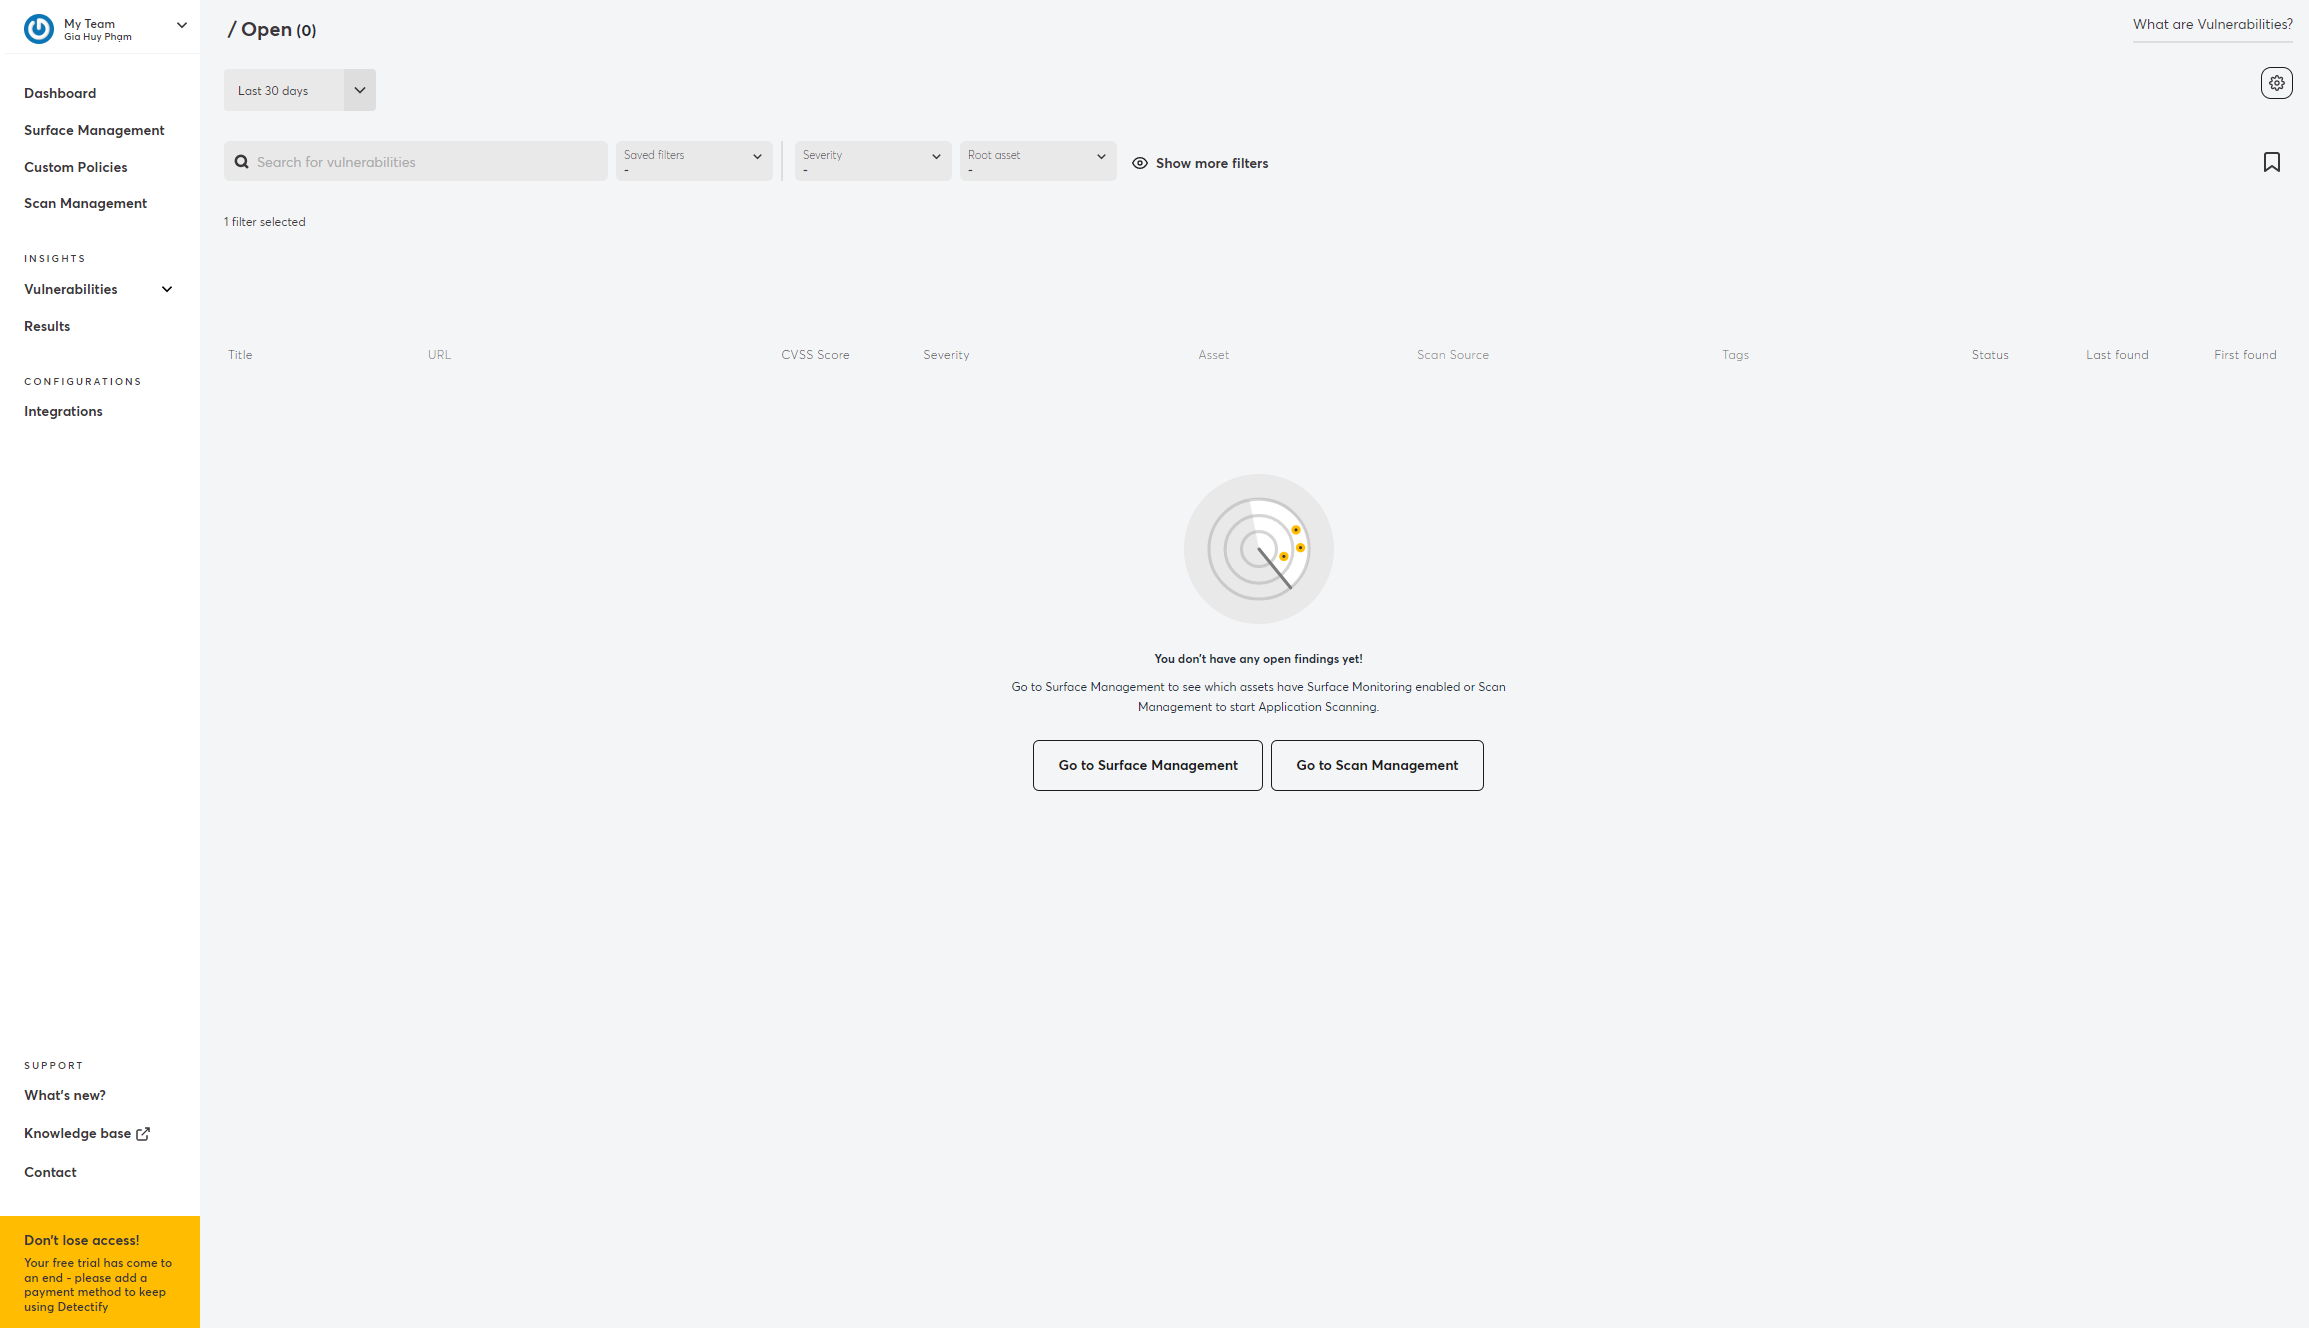
\includegraphics[width=\textwidth]{applied-thesis-chapters/chapter-1/detectify.com_app_vulnerabilities.png}
    \caption{Màn hình sau khi đăng nhập hệ thống Detectify}
\end{figure}

\subsection{“StackHawk” do StackHawk Inc. phát triển}

\tab Được thành lập vào năm 2019 tại Mỹ.
Nền tảng cung cấp chức năng tìm lỗ hổng các ứng dụng dựa trên OWASP ZAP.
Nền tảng cung cấp các chức năng quản lý như tự động quét trên mỗi PR, cung cấp tài liệu hỗ trợ sửa lỗi tìm được tương ứng, tương tác được với nhiều ứng dụng, hệ thống khác như quản lý mã, quản lý dự án, quản lý lỗi, thông báo, tự động.
Nền tảng cung cấp đầy đủ các bản mã mẫu hướng dẫn sử dụng, tài liệu thông tin và hướng dẫn.
Đồng thời cũng có hỗ trợ trực tiếp cho ứng dụng OWASP ZAP.

\begin{figure}[H]
    \centering
    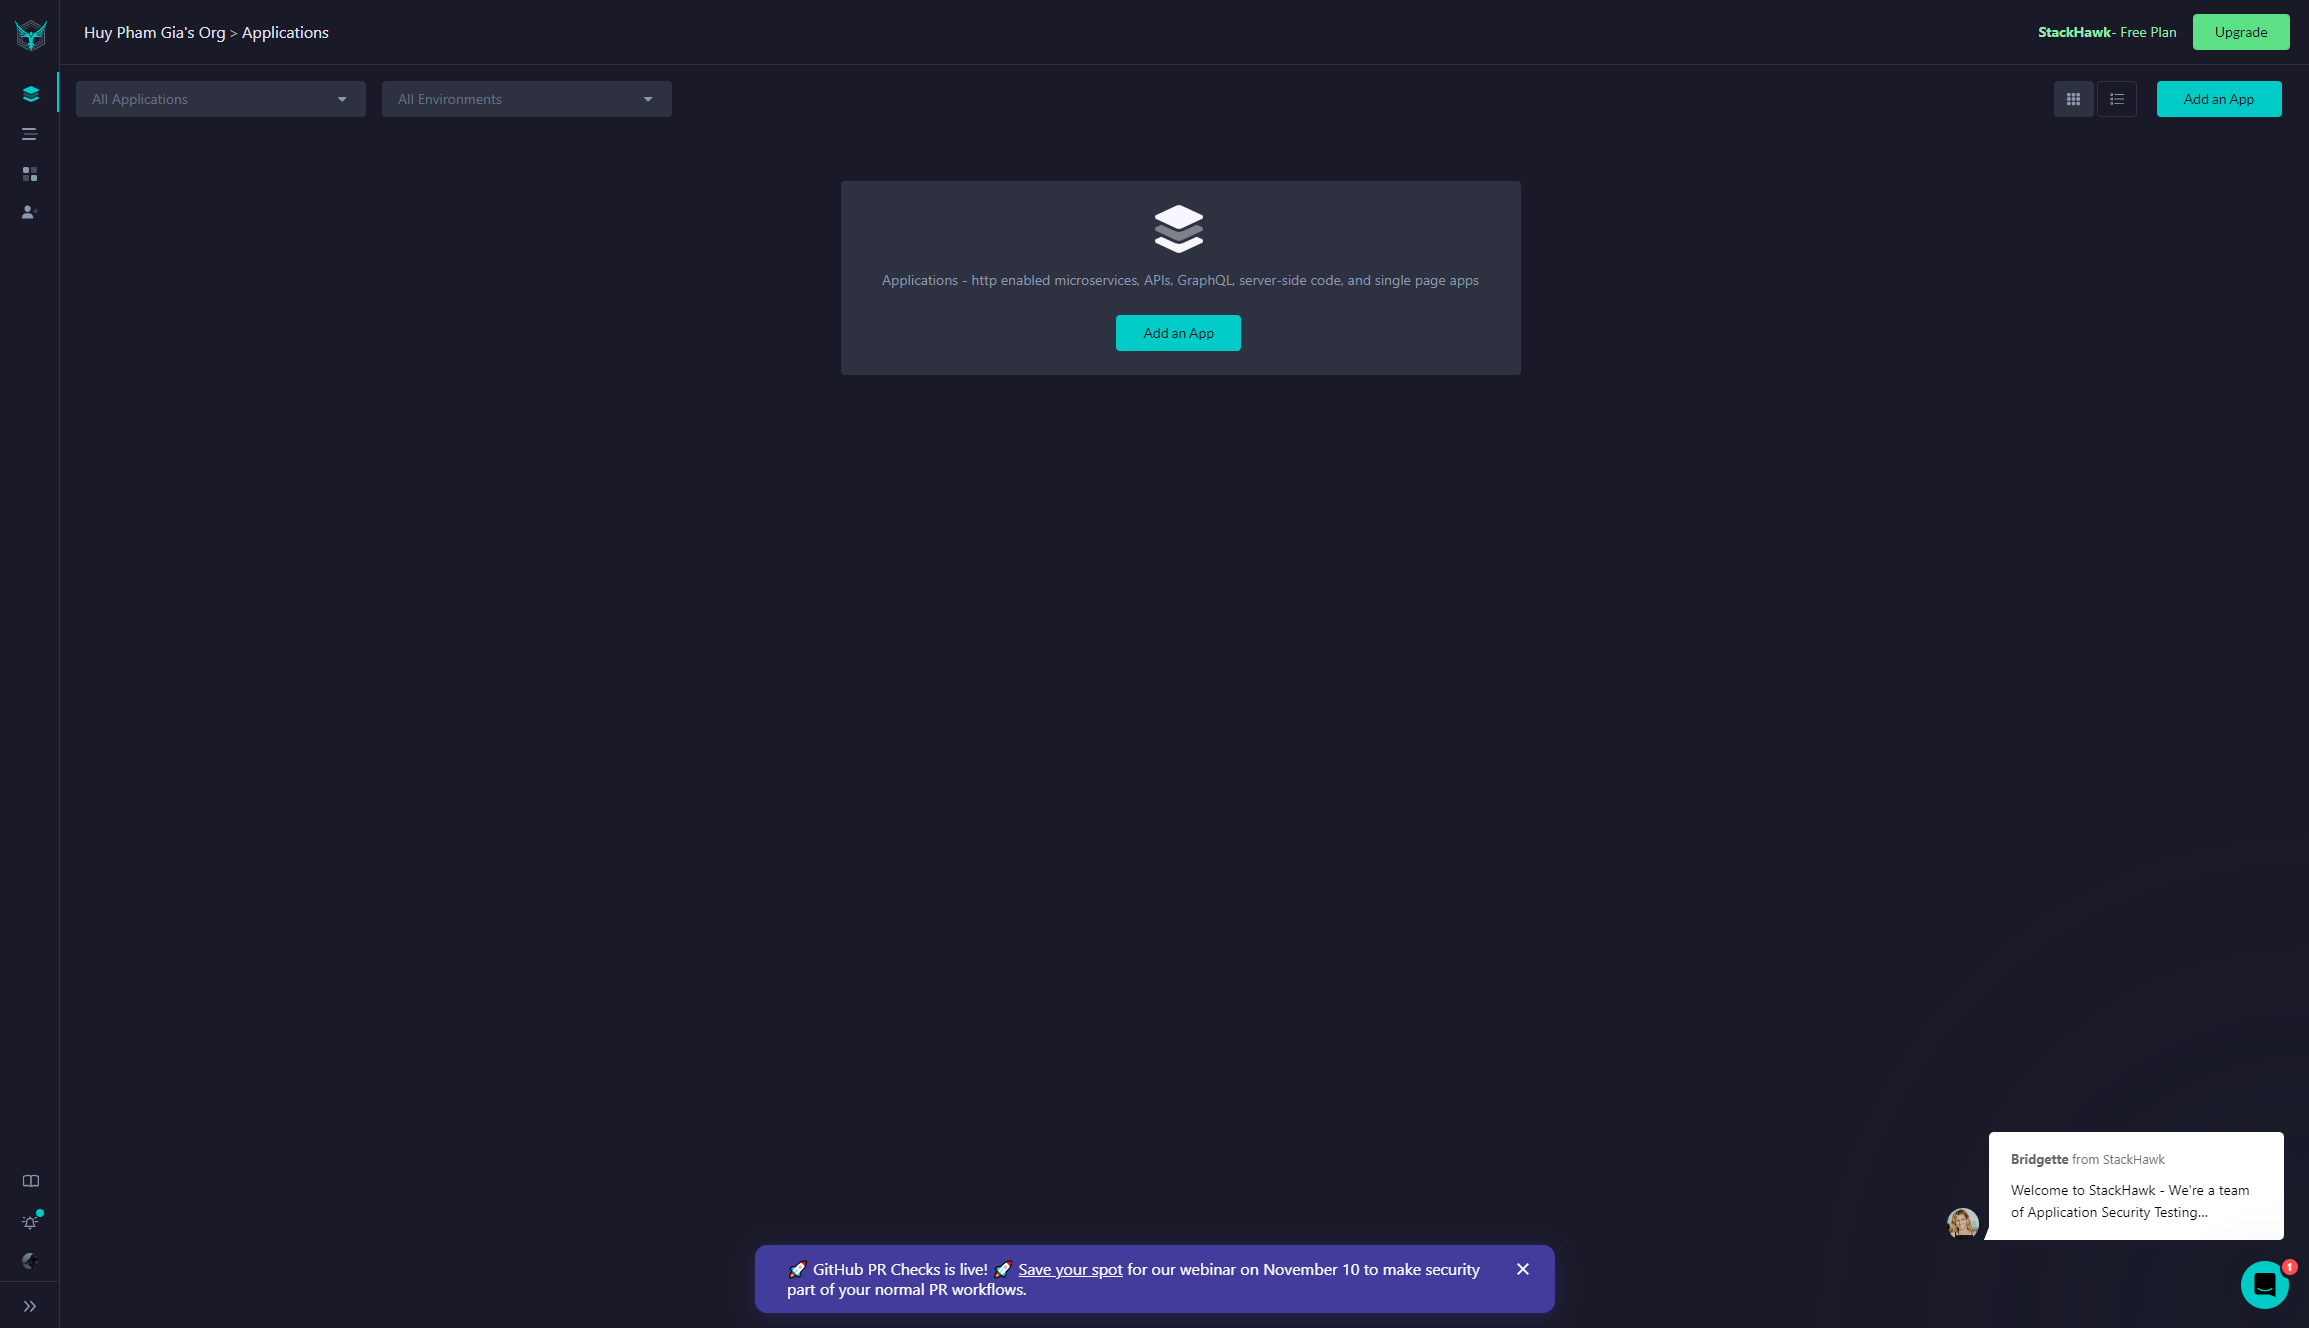
\includegraphics[width=\textwidth]{applied-thesis-chapters/chapter-1/app.stackhawk.com_applications.png}
    \caption{Màn hình sau khi đăng nhập hệ thống StackHawk}
\end{figure}

\subsection{“HostedScan Security” do HostedScan LLC phát triển}

\tab Được thành lấp vào năm 2019 tại Mỹ.
Nền tảng cung cấp nhiều loại quét như OWASP ZAP, Nmap, SSLyze.
Nền tảng có API riêng hỗ trợ cho việc sử dụng, nhúng các chức năng của nền tảng vào các ứng dụng, nền tảng khác.
Hỗ trợ hẹn lịch quét, báo cáo đầy đủ thông tin chi tiết và các tác vụ thông báo, tương tác qua email nhanh chóng.

\begin{figure}[H]
    \centering
    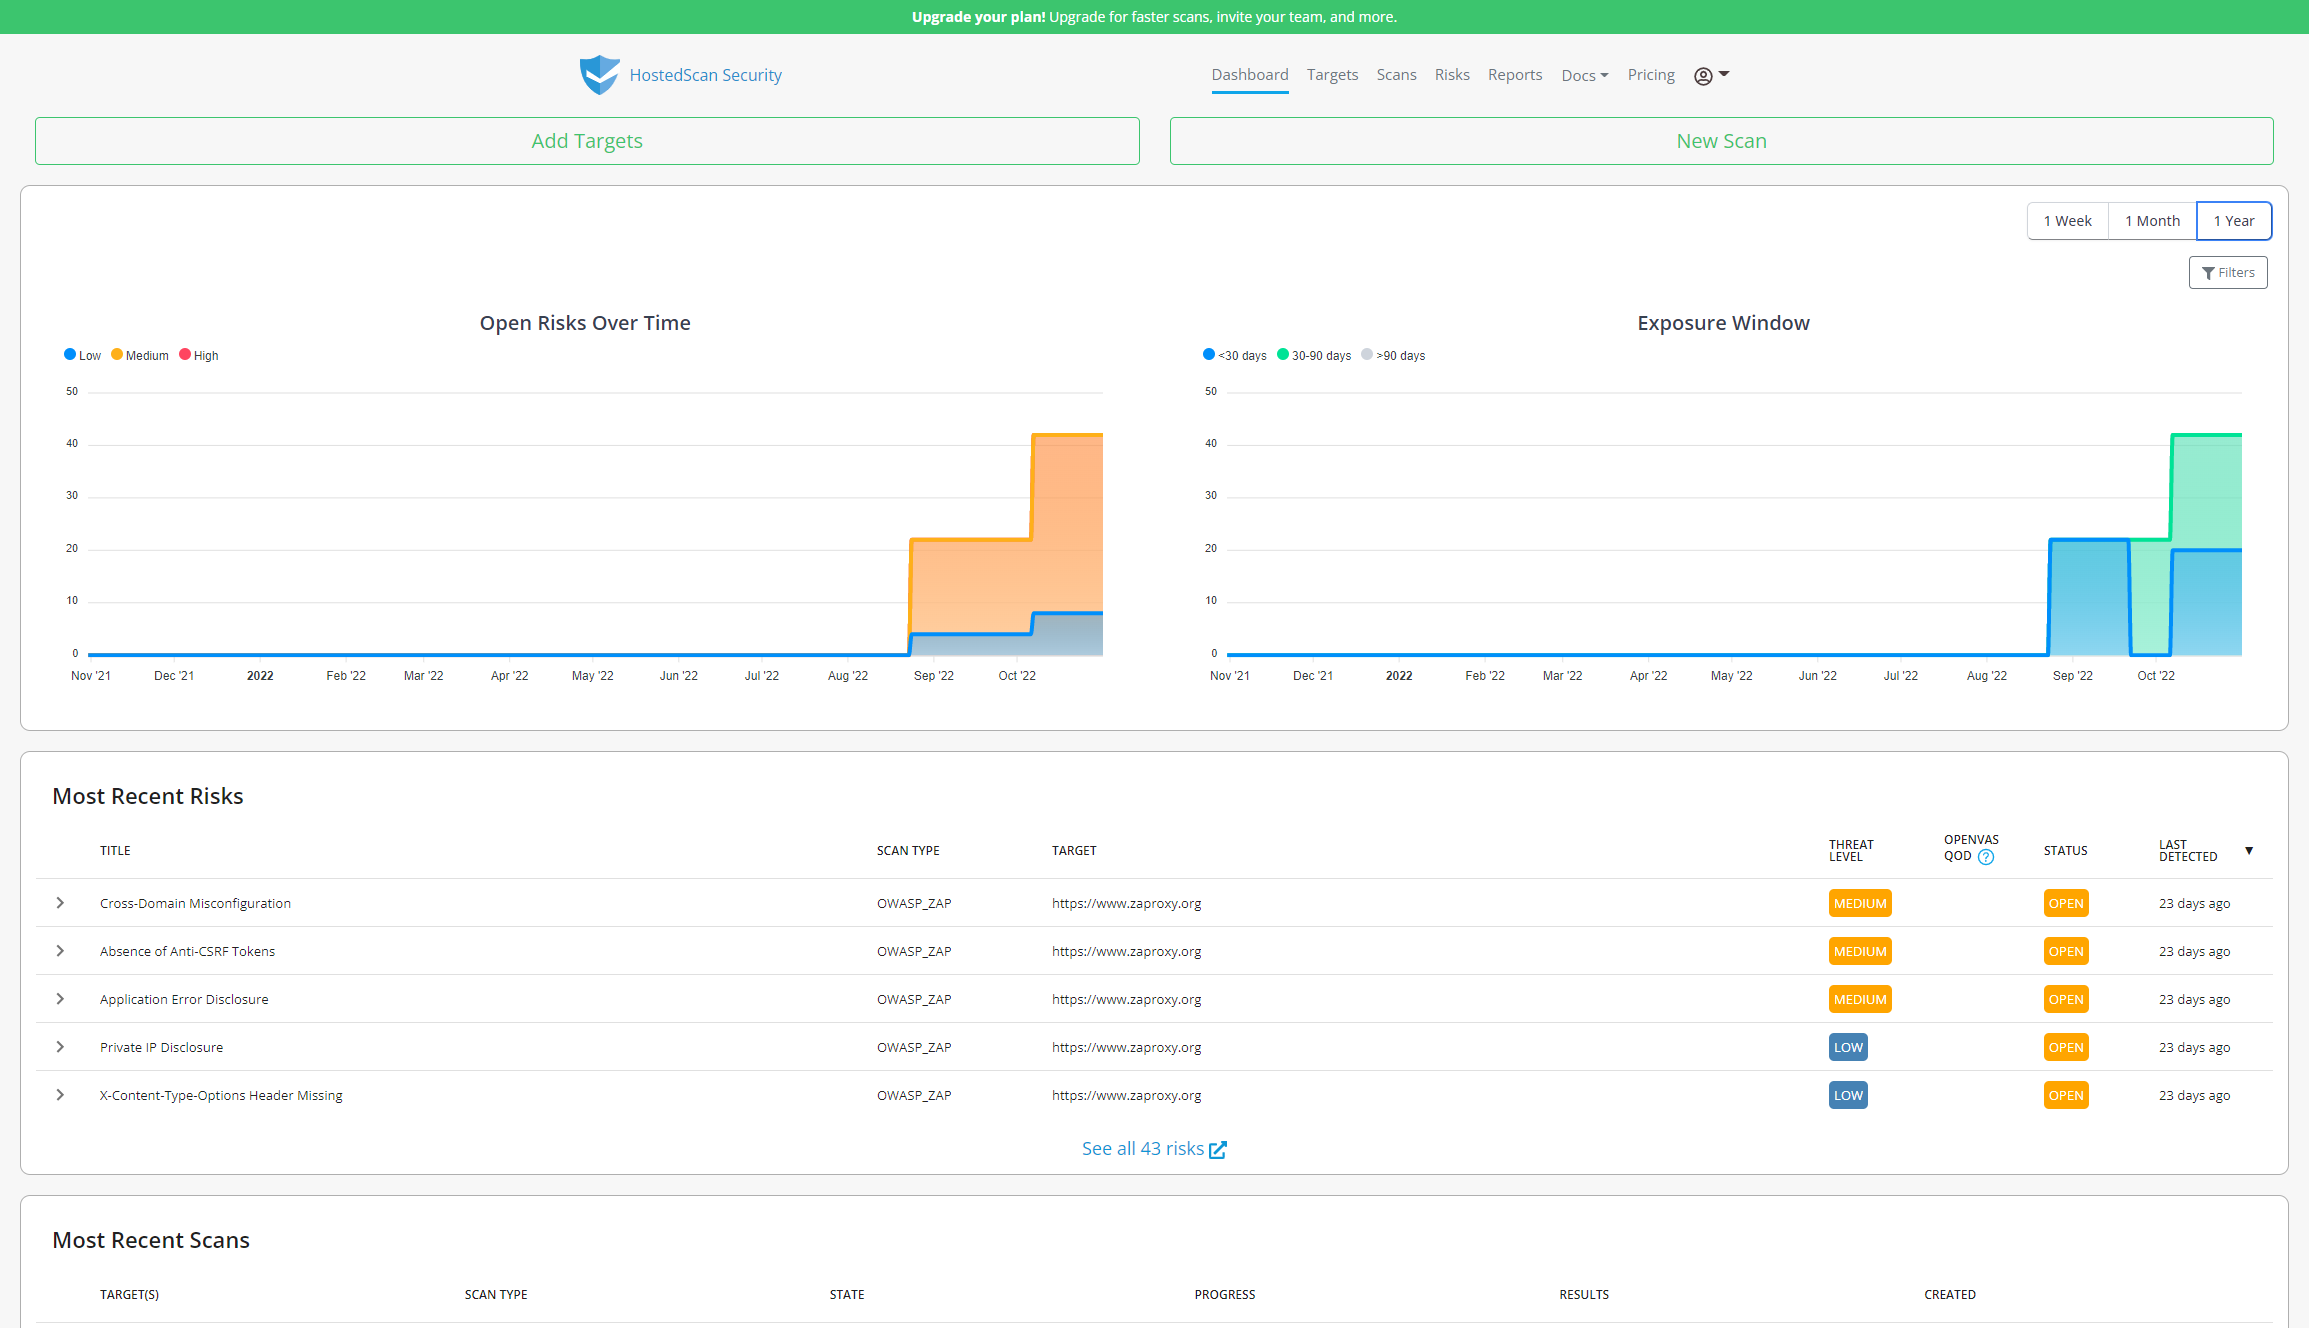
\includegraphics[width=\textwidth]{applied-thesis-chapters/chapter-1/hostedscan.com_dashboard.png}
    \caption{Màn hình sau khi đăng nhập hệ thống HostedScan Security}
\end{figure}

\subsection{So sánh nhận xét 3 hệ thống}

\begin{tabularx}{\textwidth}{|>{\hsize=0.2\hsize\centering\let\newline
    \\\arraybackslash}X|>{\hsize=0.4\hsize\raggedright\let\newline
    \\\arraybackslash}X|>{\hsize=0.4\hsize\raggedright\let\newline
    \\\arraybackslash}X|}
    \hline
    \thead{Hệ thống}
     &
    \thead{Ưu điểm}
     &
    \thead{Khuyết điểm}
    \\
    \hline
    Stack Hawk
     &
    - Tự động quét trên mỗi PR hoặc trong CI/CD.
    \newlinecontenttable
    - Quản lý thông tin kết quả quét, giao diện tường minh, dễ sử dụng.
    \newlinecontenttable
    - Đề xuất liên kết chứa thông tin sửa lỗi tìm được.
    \newlinecontenttable
    - Tích hợp được với những công cụ quản lý khác có sử dụng CI/CD như: Jira Sotfware, Gitlab, Github Action, Azure Pinelines, Jenkins, Travis CI,\dots
    \newlinecontenttable
    - Tài liệu hướng dẫn đầy đủ, chi tiết.
     &
    - Cần cấu hình pineline (.yml, .yaml).
    \newlinecontenttable
    - Cần Docker image đã build xây dựng sẵn.
    \newlinecontenttable
    - Kích hoạt quét bằng command line ở máy local. Cấu hình kích hoạt quét gồm nhiều bước.
    \newlinecontenttable
    - Dùng thử một lần mỗi ngày.
    \\
    \hline
    Hosted Scan
     &
    - Hỗ trợ các loại quét khác như Nmap, OpenVas, SSL/TLS.
    \newlinecontenttable
    - Hẹn thời gian đặt lịch quét.
    \newlinecontenttable
    - Đề xuất liên kết chứa thông tin sửa lỗi tìm được.
    \newlinecontenttable
    - Thông tin scan đầy đủ. Giao diện đơn giản.
     &
    - Kết quả scan dường như là dữ liệu gốc, không được xử lý.
    \newlinecontenttable
    - Dùng thử 10 lần mỗi tháng.
    \\
    \hline
    Detectify
     &
    - Tích hợp với các công cụ khác như: Slack, Jira, Zapier,…
    \newlinecontenttable
    - Đề xuất liên kết chứa thông tin sửa lỗi tìm được.
     &
    - Chi phí sử dụng cao.
    \newlinecontenttable
    - Cần phải cấu hình bên trong ứng dụng và triển khai để xác nhận chính chủ phức tạp, có thể không thành công.
    \newlinecontenttable
    - Không theo dõi được quá trình, tiến độ quét.
    \\
    \hline
    \caption{Bảng đánh giá chức năng giữa các hệ thống}\label{dummy-1}\\
\end{tabularx}


\section{Lý do lựa chọn đề tài}

\tab Trong thời đại ngày nay, các ứng dụng web phát triển với tốc độ nhanh chóng với số lượng, chất lượng và kích thước.
Tuy nhiên, điều này cũng làm tăng nguy cơ lỗ hổng bảo mật bị khai thác, phát hiện và lợi dụng nhiều hơn.
Gây ra nhiều nguy cơ tiềm ẩn cho ứng dụng, đội ngũ phát triển, đơn vị quản lý và chính bản thân người sử dụng ứng dụng.
Vì thế, việc tìm kiếm và khắc phục các lỗ hổng bảo mật trở thành thách thức không nhỏ, đặc biệt đối với các ứng dụng vừa và nhỏ.
\par

Mặc dù trên thị trường đã xuất hiện nhiều công cụ hỗ trợ kiểm tra, phát hiện và khắc phục lỗ hổng bảo mật cho ứng
dụng web, tuy nhiên các công cụ này thường yêu cầu nhiều bước cài đặt phức tạp hoặc chi phí sử dụng cao, khiến cho nhiều người dùng gặp khó khăn trong việc tiếp cận và sử dụng.
\par

Do đó, nhóm chúng em muốn tạo ra một hệ thống tự động tìm kiếm lỗi bảo mật ứng dụng web dựa trên nền tảng ZAP để hỗ trợ việc tìm kiếm và sửa chữa các lỗ hỗng bảo mật dễ dàng hơn.
Nhắm đến kết quả tạo ra một hệ thống dễ dàng sử dụng, dễ tiếp cận và nhanh chóng.

\section{Mục tiêu thực hiện}

Nhóm chúng em xác định rõ các mục tiêu cần đạt được khi thực hiện luận văn như sau:

\begin{itemize}
    \item Trình bày lý do xây dựng hệ thống tự động tìm kiếm lỗi bảo mật ứng dụng web dựa trên nền tảng OWASP ZAP.
    \item Trình bày các tính năng cơ bản của 3 ứng dụng tìm kiếm lỗi bảo mật ứng dụng web hiện có và nêu ra các khuyết điểm của các ứng dụng.
    \item Trình bày tóm tắt thông tin về các lỗi bảo mật ứng dụng web thường gặp.
    \item Xây dựng ứng dụng web tự động tìm kiếm lỗi bảo mật ứng dụng web với các chức năng:
          \begin{itemize}
              \item Quản lý tài khoản, các mục tiêu tìm kiếm và kết quả tìm kiếm.
              \item Quét các lỗi bảo mật với ZAP.
          \end{itemize}
    \item Viết 120 trang luận văn theo luồng logic trình bày trong tài liệu “Hướng dẫn thực hiện luận văn” mà giáo viên cung cấp, theo đúng chuẩn nhà trường yêu cầu và trích dẫn tài liệu tham khảo một cách chi tiết, đầy đủ.
\end{itemize}

\section{Phạm vi đề tài}

\tab Mục tiêu chính của đề tài “Hệ thống tự động tìm kiếm lỗi bảo mật ứng dụng web dựa trên nền tảng OWASP ZAP” là hướng tới sự dễ dàng và nhanh chóng tìm kiếm lỗi bảo mật ứng dụng và quản lý kết quả sau khi quét.
Vì vậy ứng dụng sẽ chú trọng phát triển các tính năng quét chính với ZAP đã đề xuất.
Và các chức năng quản lý cơ bản của nền tảng như quản lý mục tiêu, quản lý phiên quét.
Tuy vậy, ứng dụng sẽ tập trung vào trực quan hóa quá trình quét và giảm thiểu các cấu hình bắt buộc khi bắt đầu một phiên quét.